%%% Copyright (C) 2020 David Beauchemin
%%%
%%% Ce fichier et tous les fichiers .tex dont la racine est
%%% mentionnée dans les commandes \include et \input ci-dessous font
%%% partie du projet «Gestion de la configuration et des résultats avec MLflow, Hydra et Poutyne
%%% - Webinaire»
%%% URL
%%%
%%% Le format et le visuel est très fortement inspiré du matériel de
%%% Vincent Goulet https://gitlab.com/vigou3/webinaire-recherche-reproductible
%%%
%%% Cette création est mise à disposition selon le contrat
%%% Attribution-Partage dans les mêmes conditions 4.0
%%% International de Creative Commons.
%%% https://creativecommons.org/licenses/by-sa/4.0/

\documentclass[aspectratio=169,10pt,xcolor=x11names,english,french]{beamer}
\usepackage{babel}
\usepackage[autolanguage]{numprint}
\usepackage{amsmath}
\usepackage{currfile}                  % nom fichier de script
\usepackage{changepage}                % page licence
\usepackage{tabularx}                  % page licence
\usepackage{relsize}                   % \smaller et al.
\usepackage{awesomebox}                % boites signalétiques
\usepackage{fancyvrb}                  % texte verbatim
\usepackage{framed}                    % env. leftbar
\usepackage{pict2e}                    % cycle travail Git
\usepackage[overlay,absolute]{textpos} % couvertures
\usepackage{metalogo}       
\usepackage{textpos}           % logo \XeLaTeX

\usepackage{fontawesome}

\usepackage{stackengine, tikz} % for stacking logo

\usepackage{svg} %for svg image also need option --shell-escape

\usepackage{dirtree}


%% =============================
%%  Informations de publication
%% =============================
\title{Gestion de la configuration et des résultats avec MLflow, Hydra et Poutyne}
\author{David Beauchemin}
\date{.. novembre 2020}

%% =======================
%%  Apparence du document
%% =======================

%% Couleurs additionnelles
\definecolor{rouge}{rgb}{1,0.31,0.26}
\definecolor{bleu}{rgb}{0.18,0.23,1}
\definecolor{couleurpolice}{rgb}{0.13,0.13,0.13}

\definecolor{link}{cmyk}{0.67, 0.66, 0, 0.71}    % liens internes
\definecolor{url}{rgb}{1,0.31,0.26}       % liens externes
\definecolor{codebg}{rgb}{0.94, 0.95, 0.95}

\colorlet{shadecolor}{codebg}

%% Thème Beamer général
\usetheme[titleformat=allcaps, numbering=none, block=transparent]{metropolis}

%% Modifications aux couleurs: fond blanc, titres en texte noir sur
%% fond blanc
\setbeamercolor{normal text}{bg=white}
\setbeamercolor{frametitle}{fg=normal text.fg, bg=}

%% Déplacer les titres vers le bas sous la décoration du gabarit CFDD
\makeatletter
\setlength{\metropolis@frametitle@padding}{4.9ex}
\renewcommand{\metropolis@frametitlestrut@start}{
	\rule{0pt}{6ex +%
		\totalheightof{%
			\ifcsdef{metropolis@frametitleformat}{\metropolis@frametitleformat X}{X}%
		}%
	}
}
\renewcommand{\metropolis@frametitlestrut@end}{}
\makeatother

%% Format de la page de titre de section;
\makeatletter

\setbeamertemplate{section page}{%
	\begin{minipage}{22em}
		\raggedright
		\usebeamerfont{section title}
		\let\hyperlink\@secondoftwo\fontsize{35}{35}\textcolor[cmyk]{0.67, 0.66, 0, 0.71}{\insertsectionhead}\par
	\end{minipage}
	\par
	\vspace{\baselineskip}
}

\makeatother

%% Polices de caractères
\newfontfamily\Overpass{Overpass}
\setsansfont{Overpass}        % police principale
\newfontfamily\OverpassSemiBold{Overpass}
[
BoldFont = *-SemiBold
]
\newfontfamily\OverpassExtraLightBold{Overpass}
[
UprightFont = *-ExtraLight,
BoldFont = *-Light
]
\newfontfamily\OverpassLight{Overpass}
[
UprightFont = *-Light,
BoldFont = *-Regular
]


\setbeamercolor{frametitle}{fg=couleurpolice}
\setbeamercolor{section in head/foot}{fg=couleurpolice}
\setbeamercolor{normal text}{fg=couleurpolice}



%% Hyperliens
\hypersetup{%
	pdfauthor = {David Beauchemin},
	pdftitle = {Gestion de la configuration et des résultats avec MLflow, Hydra et Poutyne},
	colorlinks = {true},
	linktocpage = {true},
	allcolors = {link},
	urlcolor = {url},
	pdfpagemode = {UseOutlines},
	pdfstartview = {Fit},
	bookmarksopen = {true},
	bookmarksnumbered = {true},
	bookmarksdepth = {subsection}}

%% Paramétrage de babel pour les guillemets
\frenchbsetup{og=«, fg=»}

%% =========================
%%  Nouveaux environnements
%% =========================

%% Environnement pour le code informatique; hybride
%% des environnements snugshade* et leftbar de framed.
\makeatletter
\newenvironment{Scode}{%
	\def\FrameCommand##1{\hskip\@totalleftmargin
		\vrule width 3pt\colorbox{codebg}{\hspace{5pt}##1}%
		% There is no \@totalrightmargin, so:
		\hskip-\linewidth \hskip-\@totalleftmargin \hskip\columnwidth}%
	\MakeFramed {\advance\hsize-\width
		\@totalleftmargin\z@ \linewidth\hsize
		\advance\labelsep\fboxsep
		\@setminipage}%
}{\par\unskip\@minipagefalse\endMakeFramed}
\makeatother

%% Environnement pour le contenu d'un fichier; alias de snugshade*.
\newenvironment{Sfile}{\begin{snugshade*}}{\end{snugshade*}}

%% =====================
%%  Nouvelles commandes
%% =====================

%% Lien externe
\newcommand{\link}[2]{\href{#1}{#2~{\smaller\faExternalLink*}}}
\newcommand{\guillemet}[1]{\guillemotleft #1 \guillemotright}

%% Simili commande \HUGE
\newcommand{\HUGE}{\fontsize{36}{36}\selectfont}

%%% =======
%%%  Varia
%%% =======

%% Longueurs pour la composition des pages couvertures avant et
%% arrière
\newlength{\banderougewidth} \newlength{\banderougeheight}
\newlength{\bandeorwidth}    \newlength{\bandeorheight}
\newlength{\imageheight}     \newlength{\imagewidth}
\newlength{\logoheight}

\begin{document}
	
	%% Style de l'entête et du pied de page
	
	%% frontmatter
	%%% Copyright (C) 2020 David Beauchemin
%%%
%%% Ce fichier et tous les fichiers .tex dont la racine est
%%% mentionnée dans les commandes \include et \input ci-dessous font
%%% partie du projet Gestion de la configuration et des résultats avec MLflow, Hydra et Poutyne
%%% - Webinaire»
%%% URL
%%%
%%% Le format et le visuel est très fortement inspiré du matériel de
%%% Vincent Goulet https://gitlab.com/vigou3/webinaire-recherche-reproductible
%%%
%%% Cette création est mise à disposition selon le contrat
%%% Attribution-Partage dans les mêmes conditions 4.0
%%% International de Creative Commons.
%%% https://creativecommons.org/licenses/by-sa/4.0/

%% Normes de présentation visuelle 2018
%%
%% - grille de 8 unités de haut
%% - 1 mesure = 1/8 d'unité
%% - bande identitaire de 1 mesure placée au bas de la 7e unité
%% - logo haut de 4 mesures avec blancs de deux mesures en haut et
%%   en bas
%% - blanc équivalent à la largeur du blason à droite du logo
%% - bande or de la largeur du logo + blanc à droite
%%
%% Dimensions du logo UL
%%
%% hauteur: 129
%% largeur totale: 312
%% largeur blason: 102
%% valeur clé: (312 + 102)/129 = 3.209302
%%
%% Dimensions de l'image
%%
%% hauteur: 55 mesures - 1pt (filet) = 54.9191919 mesures
%% largeur: 160mm
%% ratio largeur/hauteur: 160/77.23

\begingroup
\TPGrid{16}{64}
\textblockorigin{0mm}{0mm}
\setlength{\parindent}{0mm}
\setlength{\imageheight}{54.9191919\TPVertModule}
\setlength{\logoheight}{4\TPVertModule}
\setlength{\bandeorwidth}{3.209302\logoheight}
\setlength{\banderougewidth}{\paperwidth}
\addtolength{\banderougewidth}{-\bandeorwidth}
\setlength{\bandeorheight}{\TPVertModule}
\setlength{\banderougeheight}{\TPVertModule}
\setlength{\textwidth}{\paperwidth}
\addtolength{\textwidth}{-2\TPHorizModule}

\def\titlefmt{%
  \bfseries\fontsize{19}{19}\selectfont%
  CONFIGURATION AND RESULTS MANAGEMENT WITH MLFLOW, HYDRA ET POUTYNE\par}
\def\webinaire{%
  \OverpassSemiBold\bfseries\fontsize{18}{18}\selectfont
  SEMINAR}
\def\datefmt{%
  \OverpassExtraLightBold\bfseries\fontsize{14}{14}\selectfont%
  JANUARY 19, 2021}

%%%
%%% Page de titre
%%%
\begin{frame}[plain]
  %% bandeau identitaire
  \begin{textblock*}{\paperwidth}[0,1](0mm,56\TPVertModule)
    \textcolor{rouge}{\rule{\banderougewidth}{\banderougeheight}}%
    \textcolor{bleu}{\rule{\bandeorwidth}{\bandeorheight}}
  \end{textblock*}

  %% identifiant «webinaire»
  \begin{textblock*}{2\TPHorizModule}(0.7\TPHorizModule,5\TPVertModule)
    \textcolor[rgb]{0.13,0.13,0.13}{\webinaire}
  \end{textblock*}

  %% titre
  \begin{textblock*}{12\TPHorizModule}(0.7\TPHorizModule,17\TPVertModule)
    \textcolor[rgb]{0.13,0.13,0.13}{\titlefmt}
  \end{textblock*}

  %% date
  \begin{textblock*}{10\TPHorizModule}(0.7\TPHorizModule,41\TPVertModule)
    \textcolor[rgb]{0.13,0.13,0.13}{\datefmt}
  \end{textblock*}
\end{frame}
\endgroup

	
	\begin{frame}{Objectives of the presentation}
		\begin{itemize}
			\item Introduce configuration and results management tools.
			\item Developing good practices.
			\item Improve your productivity.
		\end{itemize}
	\end{frame}
	
	\begin{frame}
		\frametitle{Votre conférencier}
		
		\begin{minipage}{0.25\linewidth}
			
\includegraphics[width=\linewidth,keepaspectratio]{img/david}
		\end{minipage}
		\hfill
		\begin{minipage}{0.70\linewidth}
			\begin{itemize}
				\item Introduced to reproducible research in 2016 (\mbox{R Markdown} et \faGit)
				\item Participation in REPROLANG of the LREC conference \cite{garneau2020robust}
				\item Active member in the development of a library to facilitate reproducibility (\link{https://poutyne.org/}{Poutyne})
			\end{itemize}
		\end{minipage}
		
		\begin{minipage}{0.25\linewidth}
			\small
			\textbf{DAVID BEAUCHEMIN} \\
			Ph.D. candidate \\
			Department of Computer Science and Software Engineering
		\end{minipage}
	\end{frame}

	\begin{frame}{On the menu}
		\begin{minipage}{0.49\linewidth}
				\centering
				\fontsize{35}{35}\faCog\vfil
				\vspace{1em}
				\normalsize Configuration management
				
		\end{minipage}
		\begin{minipage}{0.49\linewidth}
				\centering
				\fontsize{35}{35}\faAreaChart\vfil
				\vspace{1em}
				\normalsize Results management
		\end{minipage}
	\end{frame}
	
	\section{The Management of a Project}
	\begin{frame}{Management of configuration parameters}
		\begin{Scode} 
			$001 \qquad$ @experiment.config \\
			$002 \qquad$ def config(): \\
			$003 \qquad$ \quad	seed = 42 \\
			$004 \qquad$ \quad	num\_runs = 10 \\
			$005 \qquad$ \quad	iteration = 0 \\
			$006 \qquad$ \quad	source\_language = "en" \\
			$007 \qquad$ \quad	target\_language = "de" \\
			$008 \qquad$ \quad 	src\_input = "path"  \# The input source embeddings \\
			$009 \qquad$ \quad 	trg\_input = "2e path" \# The input target embeddings \\
			$010 \qquad$ \quad 	other\_input = "3e path" \# Commentaire pas clair \\
			$\:\:\: \qquad$ \quad   $\vdots$ \\
			$395 \qquad$ \quad   $n$-th parameters \\
		\end{Scode}
	\end{frame}

	\begin{frame}{Management of configuration parameters}
		\centering
		\uncover<1->{\begin{minipage}{0.24\linewidth}
				\centering
				\normalsize Which one does that again?
		\end{minipage}}
		\uncover<2->{\begin{minipage}{0.24\linewidth}
				\centering
				\normalsize Which ones necessarily go together?
		\end{minipage}}
		\uncover<3->{\begin{minipage}{0.24\linewidth}
				\centering
				\normalsize Which ones are really essential?
		\end{minipage}}
		\uncover<4->{\begin{minipage}{0.24\linewidth}
				\centering
				\normalsize How to organize them?
		\end{minipage}}
	\end{frame}

	\begin{frame}{Results Management}
		\begin{Scode}
			\dirtree{%
			.1 .
			.2 res\_1.txt.
			.2 res\_2.txt.
			.2 res\_3.txt.
			.2 res\_4.txt.
			.2 res\_5\_good.txt.
			.2 res\_5.txt.
			.2 res\_6\_fix\_a.txt.
			.2 $\vdots$.
			.2 $n$-th results file.
		}
		\end{Scode}
	\end{frame}

	\begin{frame}{Results Management}
		\centering
		\uncover<1->{\begin{minipage}{0.24\linewidth}
				\centering
				\normalsize Which configuration (already) used?
		\end{minipage}}
		\uncover<2->{\begin{minipage}{0.24\linewidth}
				\centering
				\normalsize Success or failure?
		\end{minipage}}
		\uncover<3->{\begin{minipage}{0.24\linewidth}
				\centering
				\normalsize Which one is the best?
		\end{minipage}}
		\uncover<4->{\begin{minipage}{0.24\linewidth}
				\centering
				\normalsize How to organize them?
		\end{minipage}}
	\end{frame}

	
	\section{The Solutions}
	
	\begin{frame}{On the menu}
		\begin{minipage}{0.49\linewidth}
			\centering
			\fontsize{35}{35}\faCog
			\vfil
			\vspace{1em}
			\normalsize Configuration management
			
		\end{minipage}
		\begin{minipage}{0.49\linewidth}
			\centering
			\tikz\node[opacity=0.5]{\fontsize{35}{35}\faAreaChart};
			\vfil
			\vspace{1em}
			\tikz\node[opacity=0.5]{\normalsize Results management};
		\end{minipage}
	\end{frame}

	\begin{frame}{Configuration management}
		\centering
		\uncover<1->{\begin{minipage}{0.32\linewidth}
				\centering
				\fontsize{35}{35}\faForward\vfil
				\vspace{1em}
				\normalsize Simple and efficient
		\end{minipage}}
		\uncover<2->{\begin{minipage}{0.32\linewidth}
				\centering
				\fontsize{35}{35}\faFlask\vfil
				\vspace{1em}
				\normalsize Facilitates experimentation
		\end{minipage}}
		\uncover<3->{\begin{minipage}{0.32\linewidth}
				\centering
				\fontsize{35}{35}\faLineChart\vfil
				\vspace{1em}
				\normalsize Scalable
		\end{minipage}}
		\note{
			On cherche une solution qui va être :
			
			simple et efficace pour gérer nos configurations,
			
			qui va faciliter l'expérimentation plutôt que la ralentir,
			
			extensible pour permettre la définition de plusieurs paramètres tout en étant concis.
		}
		
	\end{frame}
	
	\begin{frame}
		\frametitle{Possible solutions}
		\centering
		\begin{itemize}
			\item Arguments (e.g. argsparse, configparser)
			\item Text file
			\item JSON
			\item YAML
			\item $\hdots$
		\end{itemize}
		\note{
			1. nice when a couple of arguments (but difficult to scale, to read and maintain)
			2. Ok to read but need to be parse
			3. Cannot have comments, ok to read, sort of structured but difficult to read with that
			4. Easy to read, comments, structured
			
			The main drawback on these approaches is the lack of hierachical logic. 
		}

	\end{frame}
	
	\begin{frame}
		\frametitle{\link{https://hydra.cc/}{Hydra}}
		\framesubtitle{\textit{A framework for elegantly configuring complex applications}}
		
		\centering
		\begin{minipage}{0.24\linewidth}
				\centering
				\fontsize{35}{35}\faIcon{osi}\vfil
				\vspace{1em}
				\normalsize \textit{Open source} and MIT license
		\end{minipage}
		\begin{minipage}{0.24\linewidth}
				\centering
				\fontsize{35}{35}\faFile\vfil
				\vspace{1em}
				\normalsize YAML structured configuration files
		\end{minipage}
		\begin{minipage}{0.24\linewidth}
				\centering
				\fontsize{35}{35}\faIcon{cubes}\vfil
				\vspace{1em}
				\normalsize Hierarchical configuration files
		\end{minipage}
		\begin{minipage}{0.24\linewidth}
			\centering
			\fontsize{35}{35}\faCogs\vfil
			\vspace{1em}
			\normalsize Configurations sweeper
		\end{minipage}
		\note{
		}
	\end{frame}

	\begin{frame}{Structured configuration}
		\begin{Scode}
			data\_loader: \\
			\quad	batch\_size: 2048 \# the batch size\\
			setting: \\
			\quad seed: 42 \\
			\quad device: "cuda:0" \\
			defaults: \\
			\quad - optimizer: SGD \\
			\quad - model: bi\_lstm \\
			\quad - dataset: canadian \\
			\quad - embeddings: fast\_text \\
			trainer: \\
			\quad num\_epochs: 1 \\
			\quad patience: 30 \\
		\end{Scode}
	\end{frame}
	
	\begin{frame}{Hierarchical configuration}
		\begin{Scode}
			\dirtree{%
				.1 conf.
				.2 config.yaml.
				.2 dataset.
				.3 canadian.yaml.
				.3 netherlands.yaml.
				.2 embeddings.
				.3 fast\_text.yaml.
				.2 model.
				.3 bi\_lstm\_bidirectionnal.yaml.
				.3 bi\_lstm.yaml.
				.3 lstm\_bidirectionnal.yaml.
				.3 lstm.yaml.
				.2 optimizer.
				.3 adam.yaml.
				.3 SGD.yaml.
			}
		\end{Scode}
	\note{Logic are grouped together and are capture in a hierarchical maners. config files/directory of config files have "one responsability".}
	\end{frame}

	\begin{frame}{Hierarchical configuration}
		optimizer: SGD
		\begin{Scode}
			optimizer: \\
			\quad lr: 0.1 \\
			\quad type: sgd \\
		\end{Scode}
	\end{frame}

	\begin{frame}{Example}
		\begin{Scode}
			@hydra.main(config\_path='conf/config.yaml') \\
			def main(cfg): \\
			\quad lr = cfg.optimizer.lr \#0.1
		\end{Scode}
	\end{frame}

	\begin{frame}{Configurations sweeper}
			
			\begin{Scode}
				python main.py --multirun task=1,2,3,4,5
			\end{Scode}
			
			\begin{Scode}
				python main.py -m 'main.x=int(interval(-5, 5))' 'main.y=interval(-5, 10)'
			\end{Scode}
		\note{Plusieurs choix de sweeper Ax, Joblib, Nevergrad}
	\end{frame}

	\begin{frame}{Bonus!}
		\begin{itemize}
			\item Automatic and customizable logging
			\item Parametric instanciation 
			\begin{Scode}
				model: \\
				\quad \_target\_: models.LSTMNetwork \\
				\quad hidden\_state\_dim: 300 \\
				\quad num\_hidden\_layer: 2 \\
				\quad dropout: 0.4 \\
			\end{Scode}
		\end{itemize}
	\end{frame}

	\begin{frame}{Example}
		\begin{Scode}
			log = logging.getLogger(\_\_name\_\_) \\
			@hydra.main(config\_path='conf/config.yaml') \\
			def main(cfg): \\
			\quad log.info("Init of the trainning") \\
			\quad \vdots \\
			\quad network = instantiate(cfg.model)
		\end{Scode}
	\end{frame}

	\begin{frame}{Negative point}
		\begin{Scode}
			hydra.utils.get\_original\_cwd()
		\end{Scode}
	\note{En raison de la journalisation automatique, le working directory change.}
	\end{frame}

	\begin{frame}{On the menu}
		\begin{minipage}{0.49\linewidth}
			\centering
			\tikz\node[opacity=0.5]{\fontsize{35}{35}\faCog};
			\vfil
			\vspace{1em}
			\tikz\node[opacity=0.5]{\normalsize Configuration management};
			
		\end{minipage}
		\begin{minipage}{0.49\linewidth}
			\centering
			\fontsize{35}{35}\faAreaChart
			\vfil
			\vspace{1em}
			\normalsize Results management
		\end{minipage}
	\end{frame}

	\begin{frame}{Results Management}
	\centering
	\uncover<1->{\begin{minipage}{0.32\linewidth}
			\centering
			\fontsize{35}{35}\faIcon{user-check}\vfil
			\vspace{1em}
			\normalsize Simple to use
	\end{minipage}}
	\uncover<2->{\begin{minipage}{0.32\linewidth}
			\centering
			\fontsize{35}{35}\faIcon{archive}\vfil
			\vspace{1em}
			\normalsize Experimental logging
	\end{minipage}}
	\uncover<3->{\begin{minipage}{0.32\linewidth}
			\centering
			\fontsize{35}{35}\faLineChart\vfil
			\vspace{1em}
			\normalsize Quick visualization of experiments
	\end{minipage}}
	\note{
		On cherche une solution qui va être :
		
		simple à utiliser et \textit{utilisateur ready},
		
		qui va journaliser \textbf{intelligemment} nos expérimentations,
		
		qui permet de visualiser rapidement nos expérimentations et les comparer.
	}
	\end{frame}

	\begin{frame}
		\frametitle{\link{https://mlflow.org/}{MLflow Tracking}}
		\framesubtitle{\textit{An open source platform for the machine learning lifecycle}}
		
		\centering
		\begin{minipage}{0.24\linewidth}
			\centering
			\fontsize{35}{35}\faIcon{osi}\vfil
			\vspace{1em}
			\normalsize \textit{Open source} and Apache 2.0 license
		\end{minipage}
		\begin{minipage}{0.24\linewidth}
			\centering
			\fontsize{35}{35}\faIcon{cogs}\vfil
			\vspace{1em}
			\normalsize Automatic logging
		\end{minipage}
		\begin{minipage}{0.24\linewidth}
			\centering
			\fontsize{35}{35}\faLineChart\vfil
			\vspace{1em}
			\normalsize Simple visualization
		\end{minipage}	
		\begin{minipage}{0.24\linewidth}
			\centering
			\fontsize{35}{35}\faIcon{cubes}\vfil
			\vspace{1em}
			\normalsize Integration with Poutyne
		\end{minipage}
		\note{
		}
	\end{frame}

	\begin{frame}{Automatic logging}
		\begin{itemize}
			\item Code version (\faGit)*
			\item Training timestamp
			\item Training success/failure
			\item Computer configuration
			\item User
		\end{itemize}
	\note{*lorsque l'on utilise MLflow project}
	\end{frame}

	\begin{frame}{Simple visualization}
		\begin{Scode}
			mlflow server -p 5000 -h 127.0.0.1 --backend-store-uri file:///absolute/path
		\end{Scode}
		\note{--backend-store-uri permet de gérer le lieu de la persistance
		-h 127.0.0.1 permet d'ouvrir le port sinon 0.0.0.0 pour un local}
	\end{frame}

	\begin{frame}{Simple visualization}
		\centering
		\begin{figure}
			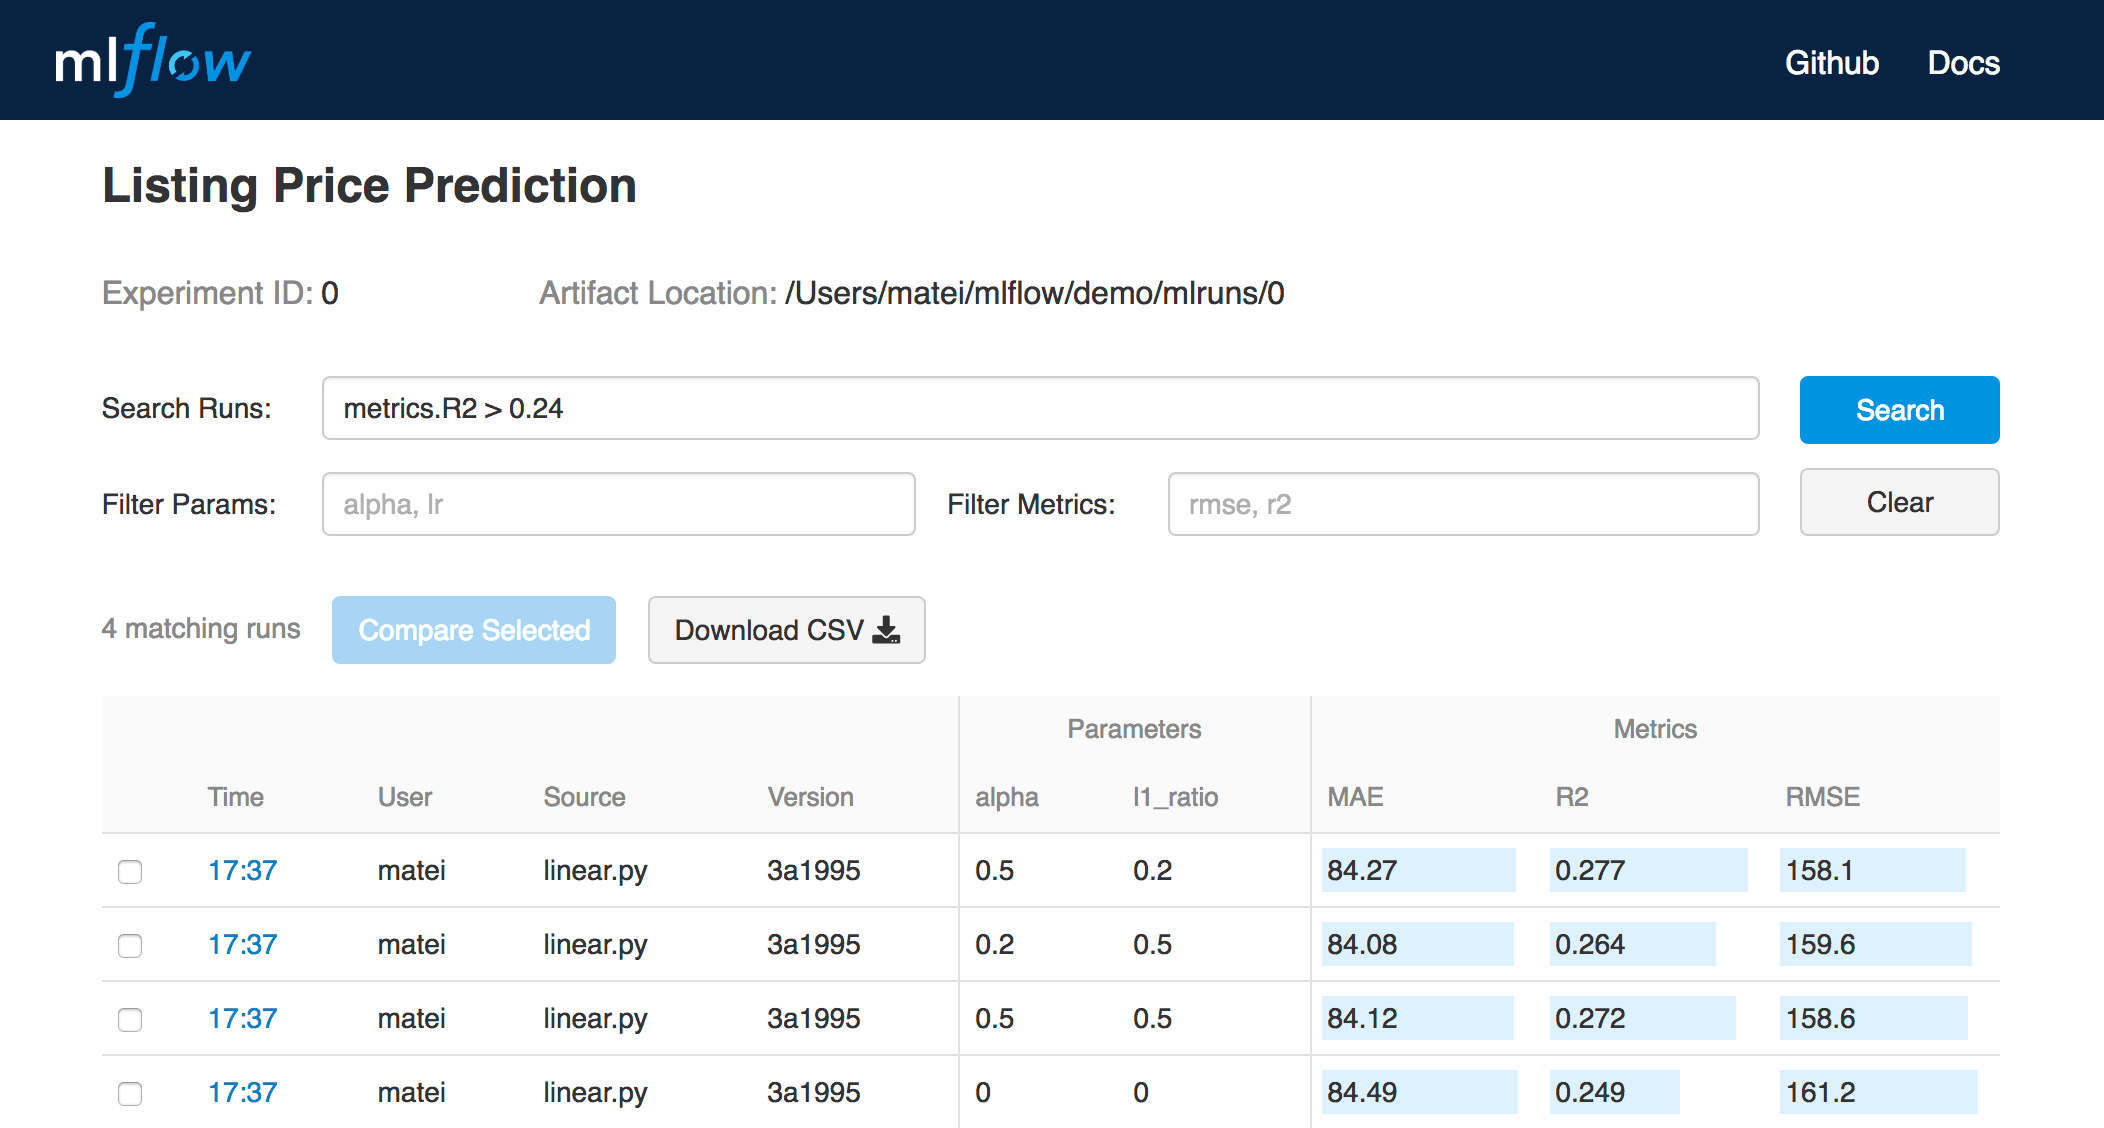
\includegraphics[width=\linewidth,keepaspectratio, height=0.7\textheight]{img/mlflow-ui.png}
			\caption{\link{https://databricks.com/blog/2018/06/05/introducing-mlflow-an-open-source-machine-learning-platform.html}{Introducing MLflow: an Open Source Machine Learning Platform}}
		\end{figure}
	\end{frame}

	\begin{frame}{Simple visualization}
		\begin{itemize}
			\item Sorting on experiments
			\item Research of experiments
			\item Queries on results
			\item Export of results
			\item Visualization of metrics
		\end{itemize}
	\end{frame}


	\begin{frame}{Integration with \link{https://poutyne.org/}{Poutyne}}
		The ''basic'' version involves manual logging 
		\begin{itemize}
			\item configuration parameters,
			\item metrics at each step and iteration,
			\item the version of the code.
		\end{itemize}
	\end{frame}

	\begin{frame}{Intégration avec \link{https://poutyne.org/}{Poutyne}}
		The solution, \color{bleu}MLFlowWriter\color{couleurpolice}, a callback allowing to journalize
		\begin{itemize}
			\item semi-automatically the configuration parameters,
			\item automatically the metrics at each step and iteration,
			\item automatically the version of the code,
			\item manually a model,
			\item automatically test metrics during a test phase.
		\end{itemize}
	\end{frame}

	\begin{frame}{Example}
		\begin{Scode}
			@hydra.main(config\_path='conf/config.yaml') \\
			def main(cfg): \\
			\quad \vdots \\
			\quad mlflow\_logger = MLFlowLogger(experiment\_name="experiment") \\
			\quad mlflow\_logger.log\_config\_params(config\_params=cfg) \\
			\quad \vdots \\
			\quad mlflow\_logger.log\_model()\\
		\end{Scode}
	\end{frame}

	\begin{frame}{Negative point}
		The documentation is not always easy to navigate.
	\end{frame}

		
	\section{What's next?}
	\begin{frame}{Présentation des résultats}
				\centering
		\begin{minipage}{0.49\linewidth}
				\centering
				\fontsize{35}{35}\faTable\vfil
				\vspace{1em}
				\normalsize Automatic generation of tables
		\end{minipage}
		\begin{minipage}{0.49\linewidth}
				\centering
				\fontsize{35}{35}\faIcon{react}\vfil
				\vspace{1em}
				\normalsize Dynamic report
		\end{minipage}
	\end{frame}
	\begin{frame}
		\centering
		\fontsize{35}{35}\faRefresh\vfil
		\vspace{1em}
		\normalsize Iterations of experiments
		\note{Développer des processus rigoureux (par essais, erreurs et journaux) et ne pas prendre tout ce qui a été discuté ici comme l'unique solution.}
	\end{frame}
	
	\begin{frame}{To go further (in order)}
		\begin{itemize}
			\item Training status notification \link{https://notificationdoc.ca/}{Notif}
			\item \link{https://cml.dev/}{Continuous Machine Learning (CML)} 
		\end{itemize}
	\end{frame}
	
	\begin{frame}
		\frametitle{Questions}
		
		\centering
		\fontsize{100}{100}
		\faQuestion
		
	\end{frame}

	%%% Copyright (C) 2020 David Beauchemin
%%%
%%% Ce fichier et tous les fichiers .tex dont la racine est
%%% mentionnée dans les commandes \include et \input ci-dessous font
%%% partie du projet Gestion de la configuration et des résultats avec MLflow, Hydra et Poutyne
%%% - Webinaire»
%%% URL
%%%
%%% Le format et le visuel est très fortement inspiré du matériel de
%%% Vincent Goulet https://gitlab.com/vigou3/webinaire-recherche-reproductible
%%%
%%% Cette création est mise à disposition selon le contrat
%%% Attribution-Partage dans les mêmes conditions 4.0
%%% International de Creative Commons.
%%% https://creativecommons.org/licenses/by-sa/4.0/

%% Normes de présentation visuelle 2018
%%
%% - grille de 8 unités de haut
%% - 1 mesure = 1/8 d'unité
%% - bande identitaire de 1 mesure placée au bas de la 7e unité
%% - logo haut de 4 mesures avec blancs de deux mesures en haut et
%%   en bas
%% - blanc équivalent à la largeur du blason à droite du logo
%% - bande or de la largeur du logo + blanc à droite
%%
%% Dimensions du logo UL
%%
%% hauteur: 129
%% largeur totale: 312
%% largeur blason: 102
%% valeur clé: (312 + 102)/129 = 3.209302
%%
%% Dimensions de l'image
%%
%% hauteur: 55 mesures - 1pt (filet) = 54.9191919 mesures
%% largeur: 160mm
%% ratio largeur/hauteur: 160/77.23

\begingroup
\TPGrid{16}{64}
\textblockorigin{0mm}{0mm}
\setlength{\parindent}{0mm}
\setlength{\imageheight}{54.9191919\TPVertModule}
\setlength{\logoheight}{4\TPVertModule}
\setlength{\bandeorwidth}{3.209302\logoheight}
\setlength{\banderougewidth}{\paperwidth}
\addtolength{\banderougewidth}{-\bandeorwidth}
\setlength{\bandeorheight}{\TPVertModule}
\setlength{\banderougeheight}{\TPVertModule}
\setlength{\textwidth}{\paperwidth}
\addtolength{\textwidth}{-2\TPHorizModule}

\def\titlefmt{%
  \bfseries\fontsize{24}{24}\selectfont%
  THANK YOU FOR \\ LISTENING!\par}
\def\webinaire{%
  \OverpassSemiBold\bfseries\fontsize{18}{18}\selectfont
  SEMINAR}

%%%
%%% Page de titre
%%%
\begin{frame}[plain]
  %% bandeau identitaire
  \begin{textblock*}{\paperwidth}[0,1](0mm,56\TPVertModule)
    \textcolor{rouge}{\rule{\banderougewidth}{\banderougeheight}}% % bande rouge
    \textcolor{bleu}{\rule{\bandeorwidth}{\bandeorheight}}           % bande or
  \end{textblock*}

  %% identifiant «webinaire»
	\begin{textblock*}{2\TPHorizModule}(0.7\TPHorizModule,5\TPVertModule)
		\textcolor[rgb]{0.13,0.13,0.13}{\webinaire}
	\end{textblock*}

  %% titre
  \begin{textblock*}{12\TPHorizModule}(0.7\TPHorizModule,17\TPVertModule)
	\textcolor[rgb]{0.13,0.13,0.13}{\titlefmt}
	\end{textblock*}
\end{frame}

\endgroup

%%% Local Variables:
%%% mode: latex
%%% TeX-engine: xetex
%%% TeX-master: "webinaire-recherche-reproductible"
%%% End:

	
	\begin{frame}[t, allowframebreaks]
		\frametitle{References}
		\bibliographystyle{apalike}
		\bibliography{GECR}
	\end{frame}
	
	
	
\end{document}
